\documentclass[12pt]{article}

\usepackage{times}
\usepackage{graphicx}
\usepackage{amsmath}
\usepackage{url}

\setlength{\textwidth}{6.5in}
\setlength{\textheight}{8.9in}
\setlength{\oddsidemargin}{0.0in}
\setlength{\topmargin}{0.05in}
\setlength{\headheight}{-0.05in}
\setlength{\headsep}{0.0in}

\newcommand{\indep}{\perp\!\!\!\perp}

\begin{document}

\begin{center}
{\bf CS 6300} \hfill {\large\bf HW08: Bayes Nets II \hfill Due April 12, 2022}
\end{center}

\noindent
Please use the \LaTeX\ template to produce your writeups.  Hand in
using gradescope.

\section{Variable Elimination}

As an anthropologist, you are studying ancient human races.  You are
also a performing artist, and have an excellent model of the way
humans invent music and dance.  The key variables are:

\begin{description}

\item[Writing (W):] Whether or not a race invented some form of writing

\item[Cold climate (C):] Whether or not the race lived in a cold weather climate

\item[Music (M):] Whether or not a race invented music

\item[Tools (T):] Whether or not a race had metal tools

\end{description}

\noindent
You model the relationships between these variables and {\bf dance (D)}
using the Bayes net below.

\begin{center}
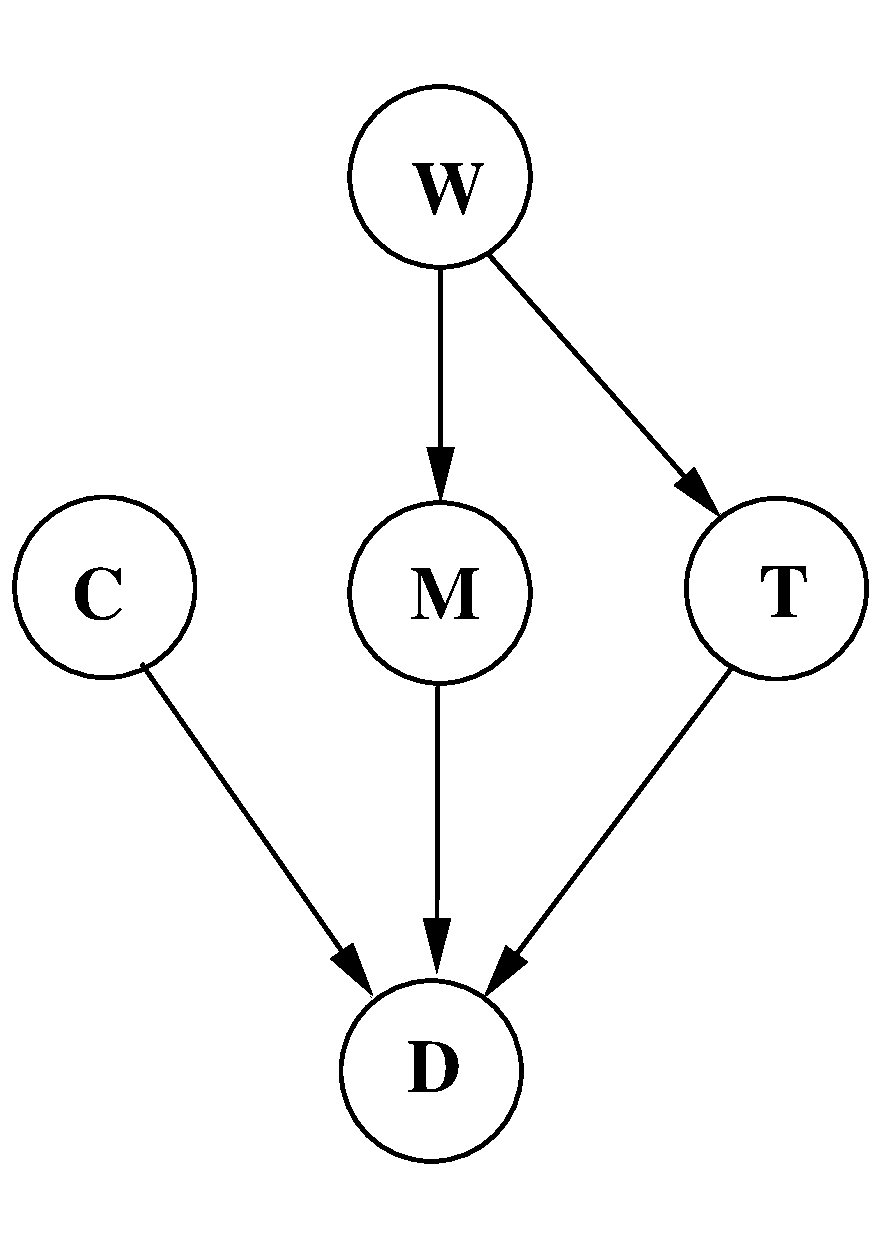
\includegraphics[height=3in]{dance1.ps}
\end{center}

\noindent
The conditional probabilities of the Bayes net are listed below.

$$\begin{array}{ccc}
\begin{array}{|c|c|c|c|c|} \hline
C  & M  & T  & D  & P(D|C,M,T) \\ \hline
+c & +m & +t & +d & 0.9 \\
+c & +m & +t & -d & 0.1 \\
+c & +m & -t & +d & 0.8 \\
+c & +m & -t & -d & 0.2 \\
+c & -m & +t & +d & 0.8 \\
+c & -m & +t & -d & 0.2 \\
+c & -m & -t & +d & 0.2 \\
+c & -m & -t & -d & 0.8 \\
-c & +m & +t & +d & 0.8 \\
-c & +m & +t & -d & 0.2 \\
-c & +m & -t & +d & 0.5 \\
-c & +m & -t & -d & 0.5 \\
-c & -m & +t & +d & 0.6 \\
-c & -m & +t & -d & 0.4 \\
-c & -m & -t & +d & 0.1 \\
-c & -m & -t & -d & 0.9 \\\hline
\end{array} &
\begin{array}{c}
\begin{array}{|c|c|c|} \hline
W  & M  & P(M|W) \\ \hline
+w & +m & 0.8 \\
+w & -m & 0.2 \\
-w & +m & 0.1 \\
-w & -m & 0.9 \\ \hline
\end{array} \\
 \\
\begin{array}{|c|c|c|} \hline
W  & T  & P(T|W) \\ \hline
+w & +t & 0.7 \\
+w & -t & 0.3 \\
-w & +t & 0.9 \\
-w & -t & 0.1 \\ \hline
\end{array}
\end{array} &
\begin{array}{c}
\begin{array}{|c|c|} \hline
W  & P(W) \\ \hline
+w & 0.9  \\
-w & 0.1  \\ \hline
\end{array} \\
 \\
\begin{array}{|c|c|} \hline
C  & P(C) \\ \hline
+c & 0.5  \\
-c & 0.5  \\ \hline
\end{array}
\end{array}
\end{array}$$

\noindent
You want to know how likely it is for a dancing, writing race to
invent music.

\begin{enumerate}

\item Write the formula to compute $P(+m | +d, +w)$ using variable elimination.

\item Now compute $P(+m | +d, +w)$.

\end{enumerate}

\clearpage

\section{Sampling}

You decide to use sampling instead.  You use prior sampling to draw
the samples below:

$$\begin{array}{|c|c|c|c|c|} \hline
W  & C  & M  & T  & D  \\ \hline
-w & +c & +m & -t & +d \\
+w & +c & -m & -t & -d \\
+w & -c & -m & +t & -d \\
+w & +c & +m & -t & +d \\
+w & +c & -m & +t & +d \\
+w & -c & -m & +t & -d \\
+w & -c & -m & -t & -d \\
+w & +c & +m & +t & +d \\
+w & +c & -m & +t & -d \\
-w & -c & -m & -t & -d \\ \hline
\end{array}$$

\begin{enumerate}

\item Based on rejection sampling using the samples above, what is the
  answer to your query $P(+m | +d, +w)$?

\item While your sampling method has worked fairly well in many cases,
  for rare cases (like a race that doesn't write) your results
  are less accurate as rejection sampling rejects almost all of the
  data.  You decide to use likelihood weighting instead.

You now wish to compute the probability that a race that has no
writing ($-w$) or dancing ($-d$) nonetheless has music ($+m$), using
likelihood weighting. I.e., you want $P(+m | -w, -d)$.

\begin{enumerate}

\item You draw four samples, using likelihood weighting.  The
  following random numbers are generated, used in the order CT.

\begin{center}
0.45 0.85 0.12 0.95 0.66 0.23 0.07 0.46 
\end{center}

Complete the following tables with the four samples.

$$\begin{array}{|c|c|c|c|c|c|} \hline
W  & C  & M  & T  & D  & \hbox{weight} \\ \hline
-w &    & +m &    & -d & \\
-w &    & -m &    & -d & \\
-w &    & -m &    & -d & \\
-w &    & +m &    & -d & \\ \hline
\end{array}$$

\item For each of these samples, indicate its weight in the same table.

\item Compute the answer to your query, $P(+m | -w, -d)$, using
  likelihood weighting with these samples.

\end{enumerate}

\end{enumerate}

\end{document}


